\section{The \netstar~Framework}
\label{sec:netstar-overview}
%Having realized about the advantages of \netstar, this section discusses the architecture of \netstar framework in detail. %is dedicated to a detailed introduction of the

\begin{figure}[!h]
  \centering
  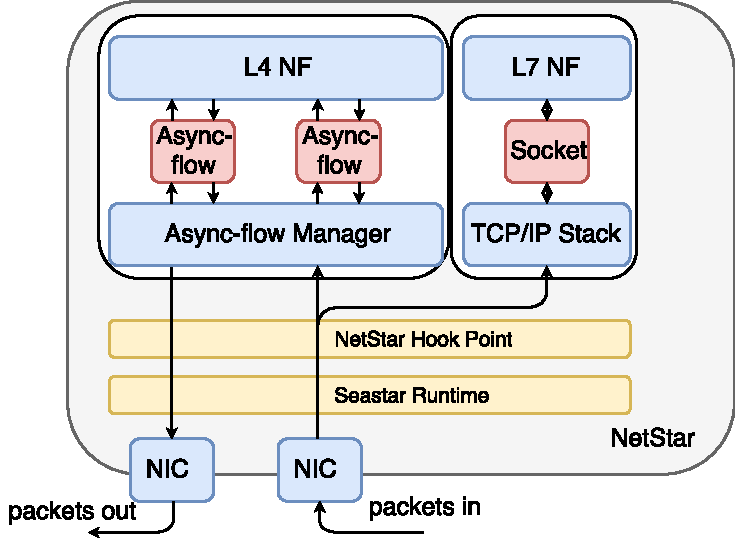
\includegraphics[width=0.6\columnwidth]{chap-netstar/figure/netstar-overvew.pdf}
  \caption{An Overview of \netstar.}
  \label{fig:overview}
\end{figure}

We design \netstar, a future/promise based programming framework for building various NFs that may carry out L4 or L7 packet processing tasks, and extensive asynchronous interactions with external services. For example, an IDS handles L4 packet processing by receiving TCP flows, reconstructing byte streams, and detecting whether they contain any malware. A proxy handles L7 application payload by forwarding application requests and responses between clients and servers. An overview of the \netstar~framework is given in Fig.~\ref{fig:overview}.


\netstar~is integrated with Seastar's runtime module, which uses DPDK to fetch packets from NIC queues directly into the user space.
\netstar~adopts a `dual-stack' design, including modules to handle packets in L4 and L7 application traffic. When \netstar~is used to implement an NF which handles L4 network packets (\ie, transport-layer packets), the hook point is configured to forward the packets received through the runtime to the async-flow manager. When \netstar~is used to implement an NF handling L7 application-level payload (\eg, a proxy), the hook point forwards the flows to the user-space TCP/IP stack. In an NF which involves both L4 and L7 traffic, the hook point classifies the packets according to their IP addresses, forwards packets whose IP addresses matches configured destination IPs to the TCP/IP stack, and others to the async-flow manager. For an IDS that carries out malware detection as in Sec.~\ref{sec:bro}, it handles L4 traffic (the TCP flows being inspected) and L7 traffic (database and MHR queries); packets carrying IP addresses of the database and MHR servers will be forwarded to the TCP/IP stack and the others to the async-flow manager.


%The TCP/IP stack of Seastar is pre-configured with an IP address. The hook point directs various L2-L4 packets that target this IP address, including ARP, ICMP TCP and UDP packets, to the Seastar TCP/IP stack for socket processing.



%\netstar is a framework  for building various NF applications that can handle various L2-L7 traffic and a variety of NFs including proxy, firewall, ids, and etc. At the lowest level, \netstar is integrated with DPDK for direct user-space packet accessing via NIC port. After packets enters \netstar, a customizable hook point classifies and dispatches packets to either (i) the user-space TCP/IP network stack or (ii) the async-flow manager, depending on the header information of the packets.

%\netstar re-use Seastar user-space TCP/IP stack to handle application-layer requests. The hook point directs TCP or UDP packets with a matching IP address to the TCP/IP stack by default. Seastar user-space TCP/IP stack exposes an interface that is similar to traditional POSIX socket. The NF application (i.e. HTTP reverse proxy \cite{}, NFs that require DNS query \cite{}) can uses the exposed socket to process application-later requests.


\textbf{Build an L4 NF.} To process L4 packets, a special interface, referred to as the {\em async-flow interface}, is designed, which consists of an async-flow manager and several async-flow objects. %After the hook point distributes matching packets to the manager,
The manager classifies received packets from the hook point into different network flows and pushes each flow to one async-flow object. The async-flow objects implement NF processing logic inside a simulated packet processing loop, using the future/promise abstraction for asynchronous operations. We will discuss our detailed design of the async-flow interface in Sec.~\ref{sec:netstar-framework}.

\textbf{Build an L7 NF.} To handle L7 application-level payload, we reuse Seastar's TCP/IP stack. The socket interface exposed by the TCP/IP stack is a modern re-implementation of the traditional POSIX socket based on the future/promise abstraction. An established TCP connection exposes a socket, through which an input stream for reading and an output stream for writing application data are available. % which facilitates asynchronous server programming for exchanging application level requests with the clients.

%\textbf{Other Usages of Seastar TCP/IP Stack.}
%Chuan: remove since it is not our contributions In \netstar, the TCP/IP stack can also be used by L2-L4 NFs built with the async-flow interface. In this way, various built-in features in the Seastar TCP/IP stack, including the DNS query interface and the RPC interface, can also be used by L2-L4 NFs. This greatly boosts the flexibility of our framework.

%\textbf{Thread Model.}
An NF built with \netstar~uses a share-nothing thread model. %, as provided by the Seastar runtime system.
Each NF runs multiple threads. Each thread is created and pined to one CPU core by the runtime. Each thread creates a complete set of modules, including the async-flow interface (one async-flow manager and multiple async-flow objects), the TCP/IP stack and the NF logic, and does not share these modules with any other thread. Incoming packets are distributed to different threads in a load balanced fashion, by configuring RSS \cite{rss} on the incoming NIC port. In this way, performance overhead associated with thread scheduling and shared resource contention is avoided. % and NFs built with \netstar~may achieve the best possible packet processing throughput.
